\documentclass[../main.tex]{subfiles}
\begin{document}
Chapter~\ref{chapter:intro} has discussed the problems which lead to the motivations of this thesis. It has also presented the objectives, the tentative solutions, and the contributions of this thesis. There are two main parts in this chapter. They are presentations about (i) related works in Section~\ref{sec:related}, and (ii) the foundation theory in Section~\ref{sec:foundtheo}. Specifically, in Section~\ref{sec:foundtheo}, models, and algorithms contributing to the making of the lightweight module on edge devices will be introduced in detail. For the purpose and scope of the thesis, four main components that make up the proposed human monitoring module on edge devices will be introduced including: (i) object detection with YOLOv5 in Section~\ref{sec:objdect}, (ii) object tracking algorithms including SORT and DeepSORT in Section~\ref{sec:objtrack}, (iii) deep metric learning with particular emphasis on the hard triplet loss function in Section~\ref{sec:deepmetric}, and (iv) MobileNetV2 architecture in Section~\ref{sec:mbv2}.

\section{Related works}
\label{sec:related}
\subsection{Person Re-Identification}


\label{sec:reidsystem}
\subsection{Edge Computing in AI}


\section{Foundation theory}
\label{sec:foundtheo}
\subsection{Object detection}
\label{sec:objdect}

Object detection technology finds applications across numerous domains including automatic traffic violation systems, identification of unfamiliar persons, digital attendance systems, and autonomous robotic vehicles. The advent of deep learning has dramatically enhanced object detection capabilities. Region-Based Convolutional Neural Networks (R-CNN) \cite{girshick2014richfeaturehierarchiesaccurate} represented one of the pioneering breakthroughs in this area, combining CNN architectures \cite{oshea2015introductionconvolutionalneuralnetworks} with region proposal mechanisms to achieve accurate object localization and classification in images. Subsequent iterations, Fast R-CNN \cite{girshick2015fastrcnn} and Faster R-CNN \cite{ren2016fasterrcnnrealtimeobject}, were developed to enhance both processing speed and detection precision compared to the original model. Despite these improvements in detection performance, the multi-step processing pipeline made these approaches impractical for real-time applications.

Modern frameworks such as Detectron2 \cite{Merz_2023} and EfficientDet \cite{tan2020efficientdetscalableefficientobject} have pushed object detection forward considerably. Detectron2 offers flexible deployment of high-performing models but demands extensive setup and typically involves computationally heavy architectures, making it unsuitable for real-time or resource-limited environments. EfficientDet provides a more practical option for devices with constrained resources, though it may struggle to meet strict real-time performance criteria.

You Only Look Once (YOLO) addresses the limitations of multi-stage detection approaches by reformulating object detection as a single regression problem. YOLO processes the entire image in one forward pass, directly predicting bounding boxes and class probabilities from full images. This unified architecture enables real-time performance while maintaining reasonable accuracy for many applications.

The YOLO family has evolved through multiple iterations, with each version improving upon speed-accuracy trade-offs. YOLOv11 \cite{khanam2024yolov11overviewkeyarchitectural}, in particular, offers several model variants ranging from nano (yolo11n) to extra-large (yolo11x) configurations. The nano variant is specifically designed for resource-constrained environments, featuring significantly reduced parameters and computational requirements while preserving essential detection capabilities.

\begin{figure}[h!]
\centering
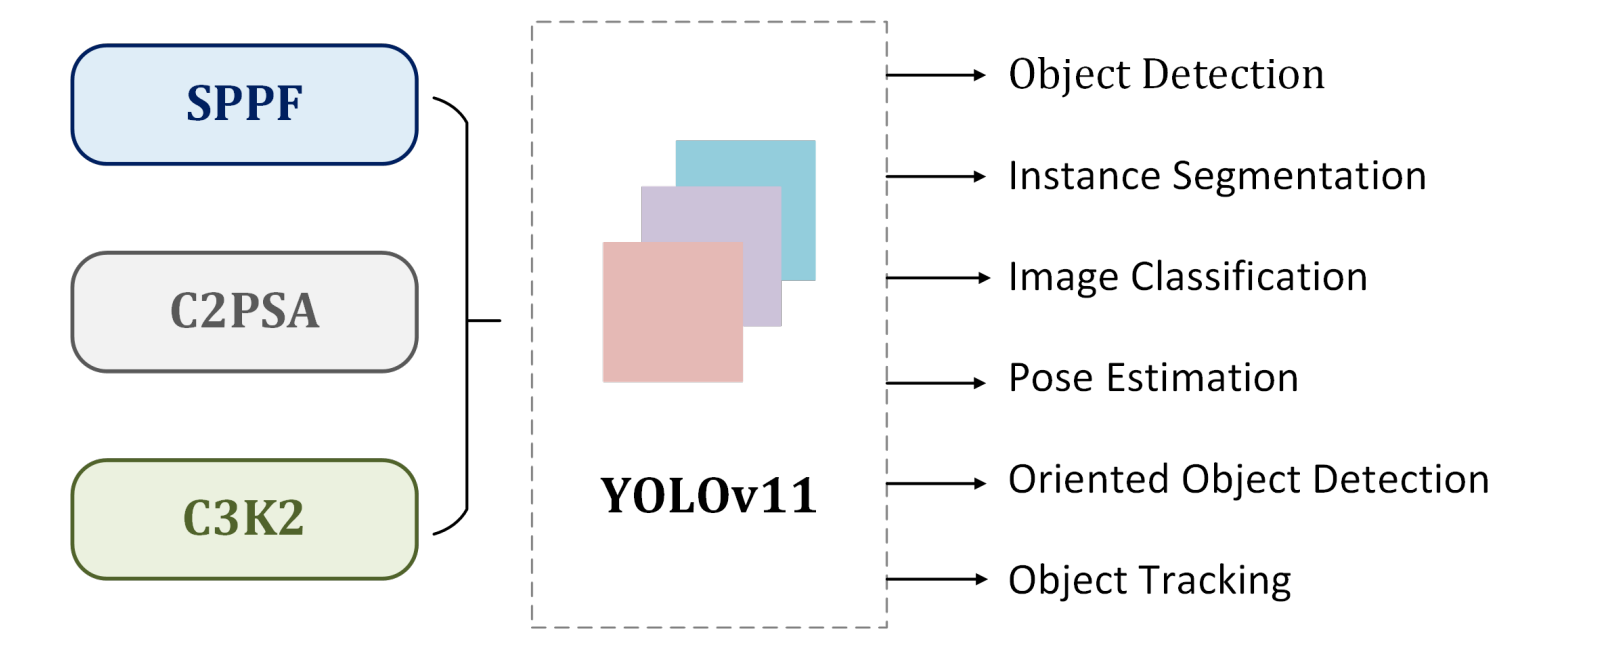
\includegraphics[width=\linewidth]{Figure/yolov11.png}
\caption{ Key architectural modules in YOLO11~\cite{khanam2024yolov11overviewkeyarchitectural}.}
\label{fig:yolov11}
\end{figure}

A significant advancement in YOLOv11 is the integration of thhe C2PSA (Convolutional
block with Parallel Spatial Attention) component, which enhances spatial attention capabilities beyond previous YOLO iterations. The C2PSA blockenables the model to focus more effectively on critical regions within images by inaplementing parallel spatial
attention mechanisms. This enhancement is particularly beneficial for detecting objects of varying sizes and positions, addressing common challengees in complex visual environments with partially occluded or small objects. The retention of the Spatial Pyramid Pooling - Fast (SPPF) blockfrom previous versions, combined with the new C2PSA component, creates a compreehensive feature processing pipeline that balances computational efficiency with enhancced spatial awareness.

For edge-based human monitoring applications, YOLOv11n provides an optimal balance between detection performance and computational efficiency. Its lightweight architecture enables deployment on edge devices for real-time person detection, serving as the foundation for subsequent tracking and Re-ID processes in distributed camera networks.

\subsection{Object tracking}
\label{sec:objtrack}
After a person is detected in the frame, that individual needed to be tracked over time in that camera. Object detection only helps us to detect desired objects in each distinct frame. To match detected bounding boxes from consecutive frames to only one entity, an object tracking algorithm is needed.

Object tracking is the process of following an object's movements and preserving its identity, even if its appearance or motion changes. Traditional methods for object tracking, such as Multiple Hypothesis Tracking (MHT)~\cite{reid1979algorithm}, create multiple tracks for each object and use a data association algorithm to select the most probable track at each time step. However, recent advances in deep learning and object detection models with neural networks have led to the rapid development of modern tracking algorithms. These algorithms are the cooperation between object detection models and motion models. Motion models use predicted bounding boxes of detection models at an interval of time step as input to estimate the motions of objects and construct entities. For instance, SORT (Simple Online and Realtime Tracking)~\cite{bewley2016simple} is a lightweight algorithm that uses the Kalman filter to predict the state of each object in each frame and the Hungarian algorithm to associate the predicted states with the detected objects in the current frame to decide which detected objects belong to which tracked objects. Even though, SORT only considers the geometric characteristics of objects. With further improvement on weaknesses of SORT, DeepSORT~\cite{wojke2017simple} incorporates a Siamese network that has been pre-trained to distinguish between individuals and add visual information to the estimation process, leading to inspiring improvements in case of occlusion where SORT fails to function. Other appearance-based methods, such as correlation filters~\cite{mekkayil2018object, bolme2010visual} and color histogram-based trackers~\cite{verges2001object, zivkovic2004like}, have also been extensively employed for object tracking.
\subsubsection{SORT}
\label{subsec:sort}
SORT is a detection-based tracking algorithm. SORT comprises four main components: detection, propagating states of tracked objects into future frames, associating existing objects with detected bounding boxes at current frames, and managing the life span of objects.

SORT takes the output results of the detection model as its input. The predicting quality of the detection model affects greatly the accuracy of SORT. Therefore, the advancement of deep learning with CNN has directly improved object detection models and indirectly boosted the performance of this tracking algorithm.

Moreover, SORT uses an estimation model to propagate states of tracked objects into future frames by using a linear constant velocity model. The model will estimate the position and velocity of each entity. When a detected bounding box is associated with a tracked object, the state of this object will be updated by this bounding box through the Kalman filter~\cite{kalman}. If no detection is associated with this tracked object, its state will be directly estimated by the linear constant velocity model without any rectifications.

To assign detections to previously identified targets, SORT will first estimate the state of each target in the current frame which is its bounding box. After that, SORT computes the distance metric between estimated bounding boxes and detections from the object detection model. This metric is IoU and the assignment will be solved by the Hungarian algorithm. This process helps the algorithm determine which detections should be assigned to which targets based on their respective bounding box geometries. Moreover, a minimum threshold is set for the assignment in order to not match tracked objects with detections that are too different from estimated states. This can prevent fault caused by short-term occlusion.

When objects appear or disappear from the image, the algorithm creates or removes identities as necessary. A new tracker is created when there is a detection that can not be matched with any existing objects. This tracker is then initialized using the detected bounding box and the velocity is set to zero. Furthermore, the newly tracked object is supervised for a few next consecutive frames where it needs to be matched with detections from the object detection model to accumulate confidence and become a new identity officially.
\subsubsection{DeepSORT}
\label{subsec:deepsort}
While SORT achieves an overall good performance, it still faces many problems especially a high number of identity switches in scenarios containing occlusions, crowded scenes, and fast-moving objects. For that reason, DeepSORT has come up with the idea to combine visual descriptors beside the velocity and motion of objects to improve data association.

Visual descriptors in DeepSORT are feature vectors that are extracted from patches in the image. These patches are cut from the original image based on the information of predicted bounding boxes. Each of these regions will be fed through a deep neural network to extract the visual feature vectors. After that, these feature vectors are normalized to obtain final visual representations of detections. Distances between tracked objects and new detections are calculated by the cosine similarity. 

DeepSORT has better accuracy compared to SORT but it has a tradeoff with inference time. Despite being not as fast as SORT, DeepSORT is still a very fast algorithm which makes it practical to be implemented on edge devices. The breakthrough concept of enhancing tracking precision by integrating both motion and visual information is incorporated into my tracking algorithm in the monitoring module to track people moving in the sight of a single camera.

\subsection{Deep metric learning}
\label{sec:deepmetric}
Metric learning is a type of machine learning that involves learning to present data points to a metric space. In this space, the distance between similar data points is expected to be small, and dissimilar data points are expected to be far apart. Metric learning can be applied to my proposed module by projecting ROI from multiple cameras or the same camera but at different timestamps of the same person to a cluster of representations close together.

Deep metric learning is a special type of metric learning which utilizes deep neural networks to automatically learn the mapping from the input space to the metric space from the data. This mapping is achieved by using a distance-based loss such as contrastive loss~\cite{hadsell2006dimensionality} or triplet loss~\cite{schroff2015facenet}. After learning a representation, it can be utilized for other tasks such as classification~\cite{deng2019deep} or clustering~\cite{li2020semi}. Many practical applications, such as face recognition and image retrieval~\cite{cao2020enhancing}, have benefited from the effectiveness of deep metric learning.

Triplet loss~\cite{schroff2015facenet} is one of the most popular loss functions in deep metric learning. It has the same objective as other types of distance-based loss functions which is shortening distances between similar data points and enlarging those of dissimilar data points. While contrastive loss~\cite{hadsell2006dimensionality} directly optimizes the above objective, triplet loss achieves that goal in an indirect way. It motivates dissimilar pairs to have distances larger than any similar pairs by a chosen margin which is illustrated in Figure~\ref{fig:triplet}. Triplet Loss tries to minimize the distance between an anchor and a positive data point which have the same label to be smaller than the distance between the anchor and a negative data point which have a different label plus the margin constant.

The triplet loss function can be defined as below:
\begin{equation}\label{eq:triplet}
    Loss = max(d(a, p) - d(a, n) + m, 0)
\end{equation}
In which:
\begin{outline}
 \1 $d$ is a distance metric between two representations such as Euclidean distance or cosine similarity.
 \1 $a$ is the anchor sample.
 \1 $p$ is the positive sample that has the same label as the anchor.
 \1 $n$ is the negative sample that has a different label as the anchor.
 \1 $m$ is the margin constant.
\end{outline}

The triplet loss method doesn't forcibly push the anchor and positive samples to be the same data point in the target space as the contrastive loss. It enables triplet loss to tolerate some intra-class variance which reflects the fact that the samples in the same class are not actually identical and that there are some outliers in datasets. Moreover, the triplet loss also doesn't optimize in an exaggerated way as contrastive loss which shortens the distance between similar pairs as much as possible. On the contrary, triplet loss only requires the distance between positive pairs to be lower than negative pairs by some margin value.

In addition, hard triplet loss is the triplet loss with the hard mining strategy~\cite{hermans2017defense}. Mining strategy is the way triplets are constructed and it helps the optimization process to converge faster and achieve better performance. In a mini-batch, this mining strategy will construct a triplet for each sample in the mini-batch by creating the corresponding hardest positive pair and hardest negative pair. In other words, it will choose the positive sample which has the maximum distance from the anchor, and the negative sample which has the minimum distance to form the triplet. All data points that were assessed are contained in a single mini-batch.

With mentioned capabilities, hard triplet loss plays a vital role in building my proposed feature extraction model. It gives the model the ability to re-identify individuals across cameras.

\subsection{MobileNetV2}
\label{sec:mbv2}
MobileNetV2~\cite{sandler2018mobilenetv2} is a lightweight neural network architecture designed for resource-constrained devices. MobileNetV2 significantly reduces the number of parameters and inference time while still achieving good accuracy. The author has introduced new bottleneck modules with inverted residual architecture.

Figure~\ref{fig:bottleneck} shows bottleneck modules of MobileNetV2 with residual connection on the left one and depth-wise layer with stride equal to two on the right one to shrink the representations. These modules take a low-dimensional tensor as input. After that, this tensor is enlarged to a high-dimensional space through a $1\times1$ point-wise convolution. This point-wise convolutional layer computes linear combinations of input channels and produces an output tensor with a preferred number of channels. Next, a $3\times3$ depth-wise convolution is applied followed by a rectified linear unit (ReLU) activation function. This convolutional layer operates by applying a distinct filter to each input channel, after which all resulting output tensors are combined into a single tensor. Finally, another $1\times1$ point-wise convolutional layer is applied to project the tensor back to a low-dimensional space. In addition, in the left module, a residual connection is used to connect two low-dimensional representations. This design improves backpropagation and costs less memory than usual residuals. On the other hand, the second module with a stride equal to two in the depth-wise layer helps to shrink the height and width of the tensor gradually. These architectures help the model to reduce a lot of parameters while maintaining accuracy. Therefore, models which are customized from MobileNetV2 have the advantages to be deployed on edge devices with limited computing capability.

This chapter has shown a detailed discussion of foundation theories. YOLOv5 is a lightweight object detection model which is appropriate for applications implemented on edge devices while retaining decent accuracy. Hard triplet loss has shown its essentiality in the problems of person Re-ID. SORT is a simple but fast tracking algorithm. On the other hand, DeepSORT proves its strength in problems that need high accuracy. In the upcoming Chapter~\ref{chapter:method}, I will discuss my development of an automatic person monitoring AI module that can be installed on edge devices. This development was informed by research results and an analysis of relevant theories and algorithms.
\end{document}